
% 
% Annual Cognitive Science Conference
% Sample LaTeX Paper -- Proceedings Format
% 

% Original : Ashwin Ram (ashwin@cc.gatech.edu)       04/01/1994
% Modified : Johanna Moore (jmoore@cs.pitt.edu)      03/17/1995
% Modified : David Noelle (noelle@ucsd.edu)          03/15/1996
% Modified : Pat Langley (langley@cs.stanford.edu)   01/26/1997
% Latex2e corrections by Ramin Charles Nakisa        01/28/1997 
% Modified : Tina Eliassi-Rad (eliassi@cs.wisc.edu)  01/31/1998
% Modified : Trisha Yannuzzi (trisha@ircs.upenn.edu) 12/28/1999 (in process)
% Modified : Mary Ellen Foster (M.E.Foster@ed.ac.uk) 12/11/2000
% Modified : Ken Forbus                              01/23/2004
% Modified : Eli M. Silk (esilk@pitt.edu)            05/24/2005
% Modified : Niels Taatgen (taatgen@cmu.edu)         10/24/2006
% Modified : David Noelle (dnoelle@ucmerced.edu)     11/19/2014

%% Change ''letterpaper'' in the following line to ''a4paper'' if you must.

\documentclass[10pt,letterpaper]{article}

\usepackage{cogsci}
\usepackage{pslatex}
\usepackage{apacite}
\usepackage{amsmath,amssymb}
\usepackage{graphicx}
\usepackage{color}
\usepackage{url}
\usepackage{todonotes}
\usepackage{mathtools}
\usepackage{stmaryrd}
\usepackage{booktabs}
\usepackage{array}
\graphicspath{{./figures/}}

%\newcommand{\url}[1]{$#1$}

\definecolor{Red}{RGB}{255,0,0}
\newcommand{\red}[1]{\textcolor{Red}{#1}}
\definecolor{Green}{RGB}{10,200,100}
\newcommand{\ndg}[1]{\textcolor{Green}{[ndg: #1]}}


 \newcommand{\denote}[1]{\mbox{ $[\![ #1 ]\!]$}}


\newcommand{\subsubsubsection}[1]{{\em #1}}
\newcommand{\eref}[1]{(\ref{#1})}
\newcommand{\tableref}[1]{Table \ref{#1}}
\newcommand{\figref}[1]{Fig.~\ref{#1}}
\newcommand{\appref}[1]{Appendix \ref{#1}}
\newcommand{\sectionref}[1]{Section \ref{#1}}

\title{Interacting pairs coordinate on lexical conventions for abstractions \\ when communicatively relevant}
 
\author{{\large \bf Robert X.D. Hawkins \textsuperscript{1}, Michael Franke\textsuperscript{2}, Kenny Smith\textsuperscript{3}, Noah D.~Goodman\textsuperscript{1}} \\
   \textsuperscript{1}Department of Psychology, Stanford University (\{rxdh,ngoodman\}@stanford.edu) \\
  \textsuperscript{2}Department of Linguistics, University of T\"ubingen (mchfranke@gmail.com)\\
  \textsuperscript{3}Centre for Language Evolution, University of Edinburgh (Kenny.Smith@ed.ac.uk)}

\begin{document}

\maketitle

%\todo[inline]{KS: title slightly under-sells the fact that they are developing a novel communication system, rather than learning a pre-existing one.  ``Hierarchically-structured lexicons evolve/emerge when hierarchical terms are communicatively relevant'' or ``Interacting pairs developed hierarchically-structured lexicons when hierarchical terms are communicatively relevant" or something like that might give more of as flavour?} 


\begin{abstract}
What drives the emergence of levels of abstraction in a communication system? Recent computational theories of language evolution suggest that the communicative demands of the environment may play a deciding role. We hypothesize that interacting pairs should more likely to lexicalize specific names (e.g. \emph{Fido}) when the context frequently requires making fine distinctions between entities; conversely, pairs should converge on a more compressed lexicon containing only words for abstract categories (e.g. \emph{dog}) when coarser contexts allow them to get away with it. We test this hypothesis by manipulating context in a repeated reference game where pairs of participants must interactively coordinate on an artificial communication system. In addition to showing qualitative differences in the levels of abstraction that emerged in participants' lexicons across different contexts, we introduce a statistical approach to probe the dynamics of the process by which abstractions gradually coalesce through interaction. These findings illuminate the local pragmatic learning mechanisms that may drive global convention formation.
\end{abstract}

\section{Introduction}
%% Set up problem
Natural languages provide speakers with remarkable flexibility in the labels they may use to refer to things \cite{Brown58_HowShallAThingBeCalled,Cruse77_PragmaticsLexicalSpecificity}. In addition to the combinatorial explosion of modifiers afforded by compositionality \cite{Partee95_LexicalSemanticsCompositionality}, we have a number of overlapping and nested terms in our lexicon. \emph{Fido}, \emph{Dalmatian}, \emph{dog}, and \emph{animal} can all reasonably be used to talk about the same entity at different levels of abstraction. How these overlapping meanings are learned, and why speakers choose different levels of specificity in different contexts, is increasingly well-understood \cite<e.g.>{XuTenenbaum07_WordLearningBayesian,GrafEtAl16_BasicLevel} but there remains a more fundamental question about the structure of our lexicon: how do abstractions become lexicalized in the first place? %And why do we have words for some abstractions but not for others?

%% Overview of big-picture optimal expressivity theory suggesting an answer
One functional answer is suggested by recent computational approaches to language evolution, which have argued that the lexical conventions of languages balance simplicity, or learnability, with the communicative needs of their users. This optimal expressivity hypothesis accounts well for the lexical distributions found in natural languages across semantic domains like color words and kinship categories \cite{RegierKempKay15_WordMeaningsEfficientCommunication}, as well as the compositional systems that emerge under iterated learning with communication in the lab \cite{WintersKirbySmith14_LanguagesAdapt, KirbyTamarizCornishSmith15_CompressionCommunication}. A key prediction is that the lexicon of a group should be sensitive to the pragmatic demands of their environment. For example, languages in warm regions ought to be more likely to collapse the distinction between ice and snow into a single word, simply because there are fewer occasions that require distinguishing between the two \cite{RegierCarstensenKemp16_WordsForSnow}. 

Still, there are several limitations to the current evidence for this hypothesis. 
First, much of the relevant evidence is observational, aggregated at the level of overall language statistics as opposed to directly manipulating the contextual conditions of individual language users. 
Second, previous experimental studies have largely focused on the outcomes of an iterated learning process, thus providing a functional argument for \emph{when} different systems may form, but have not provided a cognitive, mechanistic account of the dynamics of the formation process in individual agents.

%% Make the case for zooming into dyadic convention formation
While globally shared conventions of a language are shaped over the multi-generational timescales of cultural evolution, contextual pressures operate on the shorter timescales of dyadic interaction. 
In a matter of minutes, communication partners coordinate on efficient but informative local conventions, or conceptual pacts, for the task at hand \cite{ClarkWilkesGibbs86_ReferringCollaborative, BrennanClark96_ConceptualPactsConversation,HawkinsFrankGoodman17_ConventionFormation}. 
To understand how \emph{languages} are globally shaped by communicative constraints, it may therefore be valuable to understand the local conventions rapidly formed by adaptive agents over the course of extended interaction.

%% Hypothesis & limitations of past studies
Under the logic of a local efficiency/informativity tradeoff, we expect that 
(1) communicative pressures for informativity should lead to the lexicalization of specific names when fine distinctions must be drawn, and that 
(2) abstractions should become lexicalized precisely when the relevant distinctions are at coarser levels of the conceptual hierarchy. 
For example, we are often called upon to make fine distinctions between people in our social circles, hence lexicalizing efficient names for each individual; when referring to green beans or paper towels, however, we can get away without such specific terms -- we are rarely called upon to disambiguate between entities. %\citeA{Wittgenstein09_PhilosophicalInvestigations}
%\todo[inline]{KS: second unrelated comment at this point. The thing I find interesting from the simplicity/expressivity trade-off perspective is that hierachical terms seem like they are a bad idea - what's the advantage of having multiple terms, and how does it overcome the cost of the increase in the size of the lexicon? Is it worth flagging that up? And does our data speak to it?} 

\begin{figure*}[t]
\begin{center}
{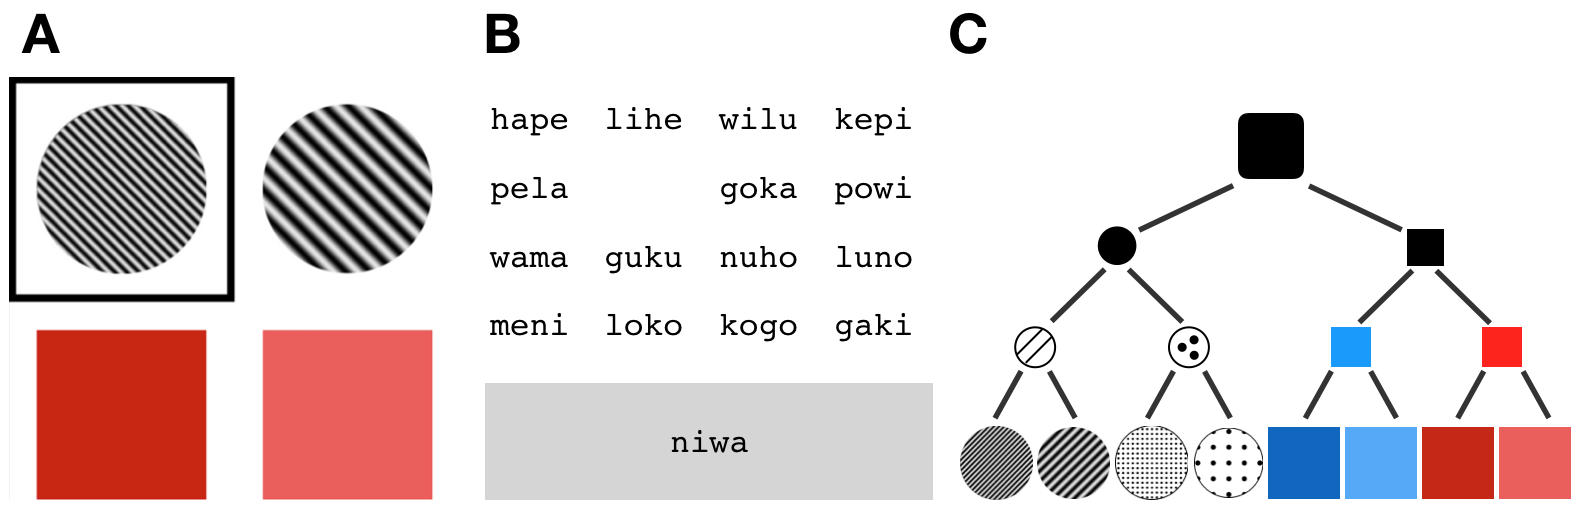
\includegraphics[scale=.65]{fig.png}}
{\caption{{(A) Example of \emph{fine} context where one of the distractors belongs to the same fine-grained branch of the hierarchy as the target (i.e. another striped circle), so any abstract label would be insufficient to disambiguate them. The target is highlighted for the speaker with a black square. (B) Drag-and-drop chat box interface. (C) Hierarchical organization of stimuli.\label{exp}}}}
\end{center}
\end{figure*}

Here, we develop an experimental paradigm and analytic approach to examine the causal factors driving the emergence of lexical conventions in real-time. 
We manipulated context in a repeated reference game where pairs of participants interactively coordinated on an artificial language from scratch  \cite<e.g.>{GalantucciGarrod11_ExperimentalSemiotics}. 
%We manipulated the pragmatic demands of context and found that abstractions only emerged when  that for the optimal expressivity hypothesis in the lexica different pairs converged on, we conducted a Bayesian Data Analysis of a rational communication model to infer the underlying lexica participants were using throughout the game. 
In both behavioral and model-based analyses, we find that abstractions only emerge when fine-grained distinctions are not necessary. We close by suggesting a learning mechanism by which pragmatic agents initially make different inferences about the lexicon their partner is using in different contexts, and therefore get away with extending terms more broadly when the context allows.  

%\ndg{this paragraph is too vague yet technical. either be more specific about design and results. or describe at the level of take-aways.}
% rational communication model allowing us to analyze not just what system they converged on but how it got there. % present a learning mechanism at the level of individual agents 
%Here, we show how the statistics of the communicative environment shape which levels of abstraction are lexicalized by interacting agents. 


% Repeated reference games 
%In this paper, however, . If there are multiple rabbits around, the travelers may need a specific conventionalized term for each; otherwise, they can achieve the same communicative success with fewer words by learning generalizations. When the pragmatics of the context allow for ambiguity in the intended level of reference, adaptive speakers can get away with extending the term more broadly. 


%% Example that sets up our specific hypothesis?

%Suppose, mixing thought experiments from \citeA{Wittgenstein09_PhilosophicalInvestigations} and \citeA{Quine13_WordAndObject}, that two travelers meet in a forest, with no language in common. One is cooking dinner, and the other agrees to help in exchange for food and shelter. What kind of micro-language do they coordinate on to solve this joint task, and how is it shaped by context? 
%To test intuitions about how pragmatics and context might affect the communication system they develop, we consider two cases. If there are multiple rabbits around, the travelers may need a specific conventionalized term for each; otherwise, they can achieve the same communicative success with fewer words by learning generalizations. 
			
\section{Experiment: Repeated reference game}

\subsubsection{Participants}

We recruited 278 participants from Amazon Mechanical Turk to play an interactive, multi-player game using the framework described in \citeA{Hawkins15_RealTimeWebExperiments}. Pairs were randomly assigned to one of three different conditions, yielding between $n=36$ and $n=53$ dyads per condition, after excluding participants who disconnected before completion.

\subsubsection{Procedure \& Stimuli}
Participants were paired over the web and placed in a shared environment containing an array of four objects (Fig. 1A) and a `chatbox' to send messages from a randomly generated vocabulary (Fig. 1B). On each of 96 trials, one player (the `speaker') was privately shown a highlighted target object and allowed to send a single word to communicate the identity of this object to their partner (the `listener'), who subsequently made a selection from the array. Players swapped roles each round and were rewarded with bonus payment when the listener successfully chose the intended object.

The objects that served as referents were designed to cluster in a fixed three-level hierarchy with shape at the top-most level, color/texture at the intermediate levels, and frequency/intensity at the finest levels (see Fig. 1C). Each communicative context contained four objects. Distractors could differ from the target at various level of the hierarchy, creating different types of contexts defined by the finest distinction that had to be drawn. We focus on two: \emph{fine} trials, where the closest distractor belongs to the same fine-grained subordinate category (e.g. another striped circle; see Fig. 1A), and \emph{coarse} trials, where the closest distractor belongs to a coarser level of the conceptual hierarchy (e.g. dotted circle instead of striped square).\footnote{Even coarser trials with super-ordinate distractors (e.g. a circle target among three square distractors) were logically possible but would have introduced several experimental confounds; we opted to leave these trial types out of our design and conduct the minimal manipulation.} Fixed arrays of 16 utterances were randomly generated in each game (constant across trials) by stringing together consonant-vowel pairs into pronounceable 2-syllable words.

Critically, we manipulated the statistics of the context in a between-subjects design to test the effect of communicative relevance on lexicalization. In the pure \emph{fine} and \emph{coarse} conditions, all targets appeared in fine or coarse contexts, respectively; in the \emph{mixed} condition, the two context types were equally likely, providing diversity in the relevant distinctions that must be drawn. Sequences of trials were constructed by randomly shuffling targets and trial types within blocks and ensuring no target appeared more than once in a row. 

In addition to behavioral responses collected over the course of the game, we designed a post-test to explicitly probe players' final lexica. For all sixteen words, we asked players to select all objects that word can refer to (if any), and for each object, we asked players to select all words that can refer to it (if any). Using a bidirectional measure allows us to check the internal validity of the lexica reported, to compare lexica across partners, and to distinguish between specific terms that apply to only one object and abstract terms that apply to all objects underneath higher nodes in the hierarchy. 

\subsection{Results}

\subsubsection{Partners successfully learn to communicate}

Although participants began with no common basis for label meanings, performing approximately at chance (25\%) on the first round, most pairs were nonetheless able to coordinate on a successful communication system over repeated interaction (see Fig. \ref{fig:accuracy}). 
\ndg{can we tell if people are actually at chance initially? maybe by comparing to a logistic regression with y-intersect pinned to 0.25?}
A mixed-effects logistic regression on listener responses with trial number as a fixed effect, and including by-pair random slopes and intercepts, showed a significant improvement in accuracy overall, $z = 14.4, p < 0.001$. 
Accuracy also differed significantly \emph{across} conditions (Fig. \ref{fig:accuracy}): adding an additional main effect of condition to our logistic model provided a significantly better fit, $\chi^2(2) = 10.8, p = 0.004$. Qualitatively, the \emph{coarse} condition was easiest for participants, the \emph{fine} condition was hardest, and the \emph{mixed} condition was roughly in between. % Looking more closely at games within the mixed condition, we found that performance on subordinate and intermediate trial types roughly mirrored the gap between the .
Finally, the (log) response time taken by the speaker to choose an utterance also decreased significantly over the course of the game, $t = -19.7, p < 0.001$, indicating that lexical mappings became increasingly established or accessible.

\begin{figure}[t]
\begin{center}
{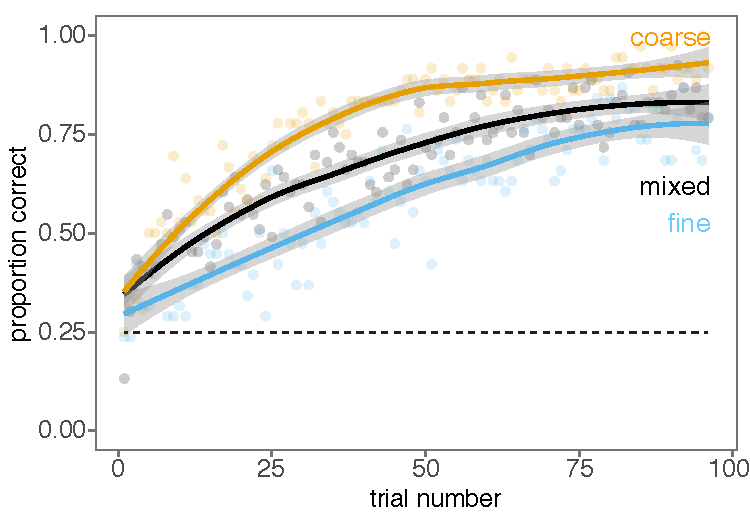
\includegraphics[scale=0.65]{accuracyByCondition_edited.pdf}}
%{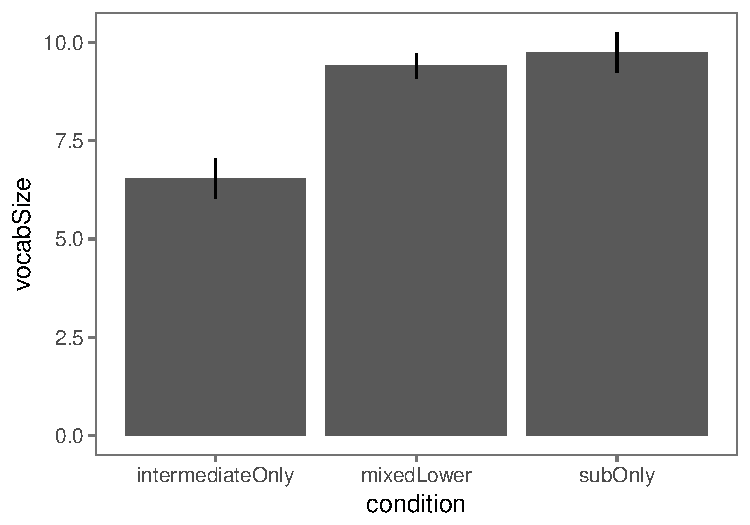
\includegraphics[scale=.64]{lexiconSize.pdf}}
{\caption{{Players learn to coordinate on a successful communication system through interaction. Each point is the mean proportion of correct responses by listeners in the given condition on the given round; smoothing curves are nonparametric regression fits.  %\todo[inline]{rdh questions: Use semantically meaningful condition codes, e.g. red/blue/purple? Is this too far aggregated from data (e.g. show error bars on each point? fit curves to individual-level binary responses instead of through group means?)}  
\label{fig:accuracy}}}}
\vspace{-.5cm}
\end{center}
\end{figure}

\subsubsection{Partners converge on similar lexica}

Another indicator of successful learning is convergence or alignment of lexica across partners in a dyad. Before computing similarity \emph{across} partners, however, we validate our dependent variable by examining the internal consistency \emph{within} an individual's post-test responses (we return to this issue in the Model-Based Results below). For each participant, we counted the number of mismatches between the two directions of the lexicon question (e.g. if they clicked the word `mawa' when we showed them one of the blue squares, but failed to click that same blue square when we shown `mawa'). In general, participants were very consistent: out of 128 cells in the lexicon matrix (16 words $\times$ 8 objects), the median number of mismatches was 2 (98\% agreement), though the distribution has a long tail (mean $= 7.3$). We therefore conservatively take a participant's final lexicon to be the \emph{intersection} of their word-to-object and object-to-word responses.

Given these estimates of each participant's lexicon, we compute the overlap across partners. Most participants aligned strongly by the end, with a median post-test overlap of 97.6\% (125 out of 128 entries). Because these matrices were extremely sparse, however, a small number of mismatches could have a large impact on performance. Overall accuracy in the game is strongly correlated with alignment: partners who reported more similar lexica at the end tended to perform better at the task ($r = 0.77$).  

\ndg{here or later: biases in which words mapped to which objects? ie kiki-boba effects.}

Despite these markers of success at the group level, individual performance was somewhat bimodal: a subpopulation of 29 games (4 from the coarse condition, 10 from the mixed condition, and 15 from the fine condition) still showed relatively poor performance, sometimes at chance, in the fourth quartile. For the subsequent analyses focusing on the content of the lexicon, we exclude games with fourth-quartile accuracy below 75\% to ensure we are examining only successful lexica.
\ndg{this was pre-planned, right? say so. more generally if this was pre-registered point out somewhere?}

\subsubsection{Contextual pressures shape the lexicon}

We predicted that contexts regularly requiring speakers to make fine distinctions among objects at subordinate levels of the hierarchy would lead to lexicalization of specific terms for each object. Conversely, when no such distinctions were required, we expected participants to adaptively lexicalize more abstract terms. One coarse signature of this prediction lies in the \emph{efficiency} of the resulting lexicon: lexicalizing abstract terms should allow participants to get away with fewer terms.

To test this prediction, we counted the number of words in the group's shared lexicon (i.e. words assigned the same meaning by both participants). We found that participants in the \emph{course} condition shared significantly smaller, more efficient lexica ($m = 4.9$ words) than participants in the \emph{mixed} and \emph{fine} conditions ($m = 7.4, t = 10.3, p <0.001$ and $m = 7.6, t = 9.5, p < 0.001$, respectively; see Fig. \ref{fig:lexiconContent}). At the same time, the smaller lexicon provided equivalent coverage of objects: the median number of objects where participants agreed on the same word or words for it was 7, 6.5, and 7, respectively.

\begin{figure*}[t]
\begin{center}
{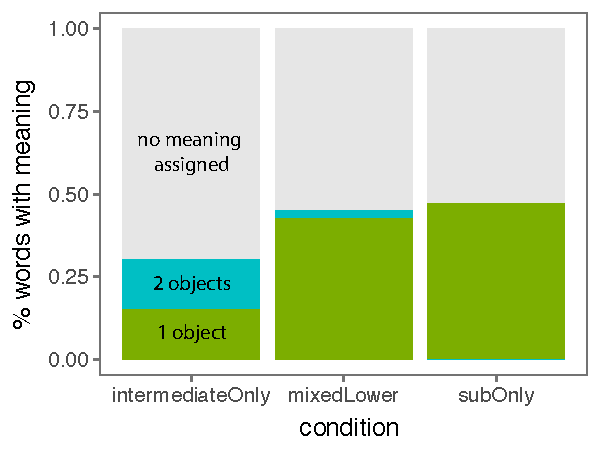
\includegraphics[scale=0.7]{lexiconContent_edited.pdf}}
{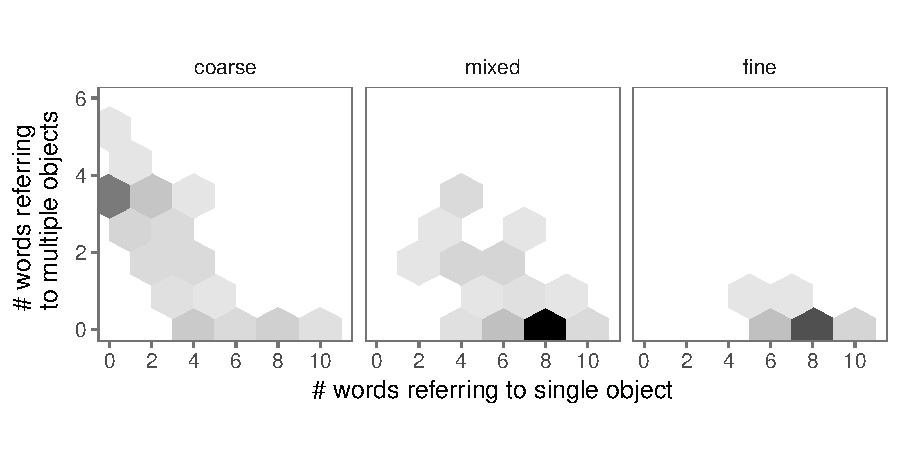
\includegraphics[scale=0.7]{fullLexiconReport.pdf}}
{\caption{{Pragmatic demands of context shape the formation of abstractions. (A) Distribution of extension sizes in lexica reported across conditions, including those with no extensions  
%\todo[inline]{KS: You'll have to explain how a word can have no extensions, but I'd be tempted to not show these in these graphs? Assuming these are uninteresting (?), showing proportion of  1 vs more-than-1 object words would make the result much clearer. Do you have this in to also show the lexicon size difference? Could show that more straightforwardly with a plot of number of words poer condition?} . 
In the \emph{fine} condition, nearly every word reported in every pair only referred to a single object; in the \emph{coarse} condition, 50\% of reported words were abstractions applying to more than one object. The \emph{mixed} condition is more similar to the \emph{fine} condition than the \emph{coarse} condition. (B) Diversity of lexica within pairs: many pairs in the \emph{coarse} condition reported a mixture of abstract and specific terms.% \todo[inline]{TODO: A/B labels; use \# words instead of \%; change axis labels in B to `'' and ``\# words referring to multiple objects'';}  
\label{fig:lexiconContent}}}}
\end{center}
\end{figure*}

If participants in the coarse condition can get away with fewer words in their lexicon, what are the meanings of the words they do have? We counted the numbers of specific terms (e.g. words that refer to only one object) and abstract terms (e.g. words that refer to multiple objects) in the post-test. We found that the likelihood of lexicalizing abstractions differed systematically across conditions (see Fig. \ref{fig:lexiconContent}A). Participants in the \emph{fine} condition reported lexica containing only specific terms, while participants in the coarse condition reported significantly more abstract terms ($m = 2.5, p < 0.001$). 

These data also reveal an interesting asymmetry in lexicon content across conditions: while abstractions are entirely absent from the \emph{fine} condition, specific terms often coexist with abstract terms in the other conditions. In the coarse condition, for instance, participants could in principle perform optimally with only four abstract terms and no specific terms. While this was the modal system that emerged (reported in the post-test by nearly 1/3 of participants), the two kinds of terms often coexisted (see Fig. \ref{fig:lexiconContent}B). Indeed, the average entropy of the distribution of abstract vs. specific terms within each participant's lexicon was highest in the coarse condition ($m = 0.20, p < 0.001$).
\ndg{`average entropy of the distribution of abstract vs. specific terms within each participant's lexicon' is a lot to swallow at once...}

\section{Model-based Analysis}

Our post-test provides some insight into the end-result of lexicalization under different communicative contexts, but understanding the \emph{dynamics} of lexicalization requires more detailed analysis of behavioral trajectories. How do lexica shift and develop over the course of interaction? 
\ndg{i think you should save the hawkins etal learning story for discussion. here you just need the basic idea that speaker-listener behavior is derived from lexicon by RSA.}
A recent cognitive model of convention formation has explained the rapid coordination on efficient but informative lexical terms as a process of mutual lexical learning \cite{HawkinsFrankGoodman17_ConventionFormation}. Each agent assumes their partner is rationally producing cooperative utterances under some latent lexicon; given initial uncertainty over the contents of that lexicon, agents can invert their model of a communicative agent to infer their partner's lexicon from their observable behavior \cite{BergenLevyGoodman16_LexicalUncertainty}. %Each individual is trying to infer the lexicon being used by their partner by observing their behavior in context. 
Listeners assume speakers are trying to be informative and parsimonious, and speakers assume listeners interpret utterances by evaluating meanings in their lexicon against objects in context \cite{FrankGoodman12_PragmaticReasoningLanguageGames,GoodmanFrank16_RSATiCS}. 

Here, we present a purely statistical model of this progression without attributing any learning mechanisms to the agent. That is, we assume that on any given round, the speaker is rationally producing utterances given some internal lexicon, and we invert a model of a pragmatic speaker to infer what that lexicon is. First, this analysis validates our post-test measures of lexical meaning against actual behavioral usage throughout the game --- if participant reports are internally consistent, the model's posterior on the last round of the game should be able to independently predict their post-test responses. Second, we can compare the time-course of lexical emergence by looking at inferences from earlier rounds of the game. Finally, because our statistical model learns from the same data that agents in principle learn from, it provides some insight into the path-dependent effects of early communicative pressures on the available meanings. %basic-level vs. subordinate-level terms, (4) measure path-dependence, e.g. how 
\ndg{does it really do that last thing?}

\subsection{Generative model}

\ndg{this section can be compressed and clarified. i think it might be better to have a (one paragraph) subsection on RSA first pointing out that this determines behavior given a lexicon. then a section describing a quartile-wise hierarchical model on lexica. avoid adding a lot of "we could have done blah".}

We begin by defining the lexicon used by participant $p$ at time $t$ as a function 
$$\mathcal{L}_p^{t} : (w, o) \rightarrow [0,1]$$ 
assigning any word-object pair a real-valued meaning in the unit interval. Assuming for simplicity that the entries are independent (we later relax this assumption), this function can be represented as a $\mathcal{W} \times \mathcal{O}$ matrix of real values $\ell_{w,o}^t \in \mathbb{R}$ mapped to the unit interval with a logistic function $f(x) = 1/(1 + e^{x})$. Our aim is to infer this sequence of values from participant behavior in the game using Bayesian data analysis techniques. 

Because observations on each round are sparse relative to the number of entries in the lexicon, we use a hierarchical Bayesian model to share statistical strength across periods of time. While more deeply hierarchical designs are possible, we simply divide the game into quartiles and assume that the lexicon $\mathcal{L}^t_p$ used by participant $p$ on round $t$ is drawn from a multi-variate Gaussian $\mathcal{N}(\mathcal{L}^{0}_p, \sigma_p^{0})$ centered at that quartile's hyper-lexicon with some fixed dispersion. To capture our uncertainty about the lexicon being used by participants (who are likely to have weak expectations for the artificial words in our experiment), we place a relatively uninformative but regularizing prior $\ell_{w,o}^0 \sim \mathcal{N}(0, 1)$ on the entries of the quartile-level lexica. 

%We capture the temporal dependence of subsequent lexica by placing a Gaussian random walk on lexical entries: the lexicon at time $t+1$ is sampled from a Gaussian distribution centered at the lexicon on the previous trial: $$\ell_{w,o}^{t+1} \sim \mathcal{N}(\ell_{w,o}^t, \sigma)$$ where sigma is a hyperparameter determining the drift rate. \todo[inline]{Is this related to the bayesian RL thing in Mathys et al, 2011?}

Finally, we must define a linking function from this underlying lexicon to the speaker utterances and listener choices we observe on each round. To capture the assumption that participants attempt to communicate pragmatically using their internal lexicon, we use the probabilistic Rational Speech Act (RSA) framework. RSA models ground out in a \emph{literal listener} agent, who uses its lexicon to directly interpret a word $w$ in context: $P_{L_0}(o_i | w, \mathcal{L}^t) \propto \mathcal{L}^t(w,o)$. A pragmatic speaker, reasoning about this listener, produces utterances by soft-maximizing a utility function taking into account the relative \emph{informativity} of saying different words in context. Formally, this informativity is given by the likelihood of the literal listener correctly interpreting the utterance to mean the intended target: $$P_{S_1}(w | o_i, \mathcal{L}) \propto \exp\{\alpha \ln P_{L_0}(o_i | w, \mathcal{L}^t)\}$$
where $\alpha$ is another hyperparameter determining the soft-max optimality of the speaker. Finally, a pragmatic listener inverts this speaker model to infer the intended referent $o_i$ given the utterance they heard $P_{L_1}(o_i | w, \mathcal{L}) \propto P_{S_1}(w | o_i, \mathcal{L}^t) P(w)$.
\ndg{collect the RSA eqs into one block, with a paragraph of description. don't need much.}

%\todo[inline]{TODO: Be explicit about how this allows us to strengthen our inferences? Needs to be cleaned up.}
%This allows us to learn about meanings of words and objects we haven't seen. e.g. suppose we hear a speaker say `mimi' to refer to one of the blue squares in the context of the other blue square. If `mimi` applied to both blue squares equally well in their lexicon, then the data would be extremely unlikely: the speaker would have avoided such an underinformative utterance. The data is much more likely under a lexicon where `mimi` only refers to the target blue square much more strongly.  Similarly, if another word in their lexicon was more informative in distinguishing these items, we assume they would have used it. Note that when the same utterance is used in a coarse trial, where only one of the blue squares is in context, it is ambiguous whether or not it can also apply to the other blue square.

These linking functions assign a fully differentiable likelihood to our dataset for any given sequence of lexica. We can therefore use mean-field variational inference \cite{RanganathGerrishBlei13_BlackBoxVariationalInference}, implemented in the probabilistic programming language WebPPL \cite{GoodmanStuhlmuller14_DIPPL}. We optimize a family of Gaussians to minimize the evidence lower bound (ELBO) which approximates the joint posterior over all lexical entries (and shared hyperparameters) used by each participant for each round in each game. 

%\begin{figure}[t]
%\begin{center}
%{\includegraphics[scale=.4]{modelSchematic}}
%%{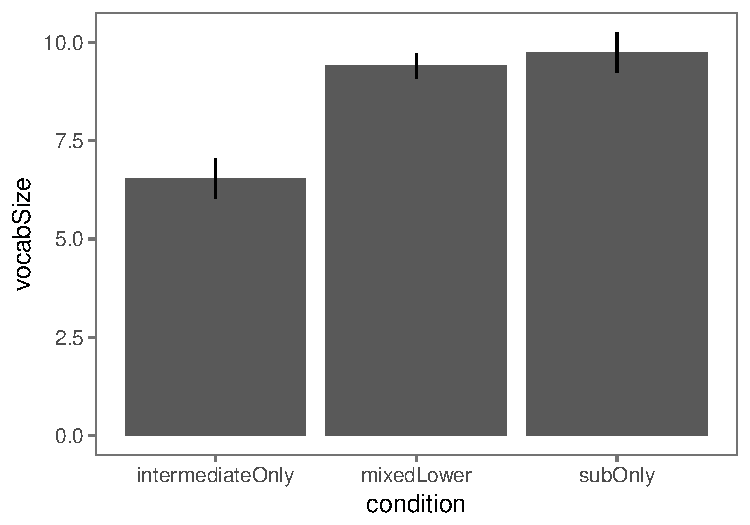
\includegraphics[scale=.64]{lexiconSize.pdf}}
%{\caption{{\footnotesize \todo[inline]{question for NDG: I wanted some kind of schematic of the model, but I'm not sure this plate notation is the best way of doing it (whether supplementing plate with a cartoon, or replacing it?)\dots Notation is kind of icky right now, too\dots this would ideally lay out very clearly the intuition behind how early contexts affect lexicon learning}  \ndg{i'd cut this. i don't think you need a bda model figure.}   \label{fig:modelSchematic}}}}
%\end{center}
%\end{figure}


\begin{figure}[t]
\begin{center}
{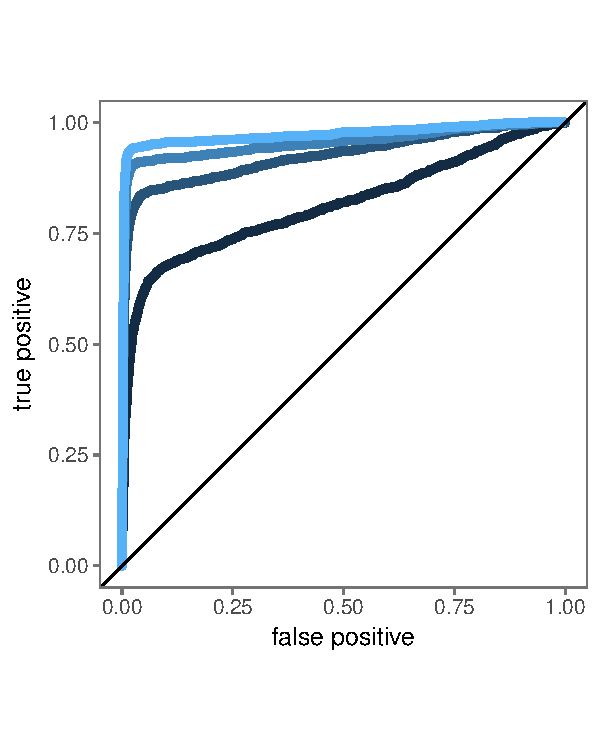
\includegraphics[scale=0.7]{modelPerformance.pdf}}
%{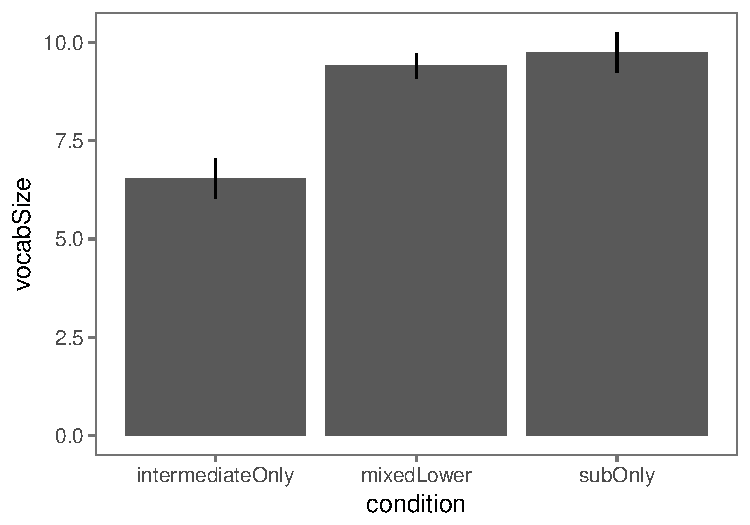
\includegraphics[scale=.64]{lexiconSize.pdf}}
{\caption{{\footnotesize \todo[inline]{TODO: directly label lines, fill bottom-right empty space with inset showing each quartile's AUC as little bar plot (e.g. 4th quarter: 0.98) \dots )}  \label{fig:postTestPrediction}}}}
\end{center}
\end{figure}

\subsection{Validating post-test responses}

We begin by showing that the lexicon learned by this model accurately predicts the post-test responses. We constructed a logistic classifier from the posterior over lexical entries on the final quartile: for each lexical entry $\ell_{o,w}$ in the $[0,1]$ interval, we calculated the marginal posterior predictive $P(\ell_{o,w} > 0.5 | \theta)$\ndg{what's $\theta$?}, giving the relative likelihood under our model of word $w$ applying to object $o$. We constructed an ROC curve by examining the hits and false alarms produced when using this predictor as we varied the discrimination threshold, and found that it predicts post-test responses with excellent accuracy (AUC: 0.98). 
\ndg{This indicates that the post-test lexicon is indeed lined to behavior as predicted by RSA, validating both the post-test measure and the BDA results.}

Furthermore, we found that the corresponding posterior predictives from earlier quartiles predicted final post-test responses less well, even though they were learned from the same number and type of behavioral observations (see Fig. 5). Still, even the classifier based on the earliest quartile performs significantly above chance, indicating that some information about the final lexicon is available from the earliest rounds. These patterns are suggestive of a path-dependent process where the lexicon gradually coalesces from initially arbitrary associations over the course of interaction. We next turn to the earliest stages of this emergence to understand this process in more detail.

\subsection{Examining early time course}

Computational models of language change distinguish between \emph{semantic broadening}, when an initially narrow word takes on a more inclusive meaning, and \emph{narrowing}, when meanings become more restrictive over time (CITE). Either of these processes could be at work in our task; we use our inferred lexica to look for signatures of these two processes. %Having validated our final-round lexicon estimates against post-test measures, we proceeded to analyze the dynamics of the lexicon over time. 
For this analysis, we elaborated our model to use an underlying feature basis to derive the lexicon instead of independent entries for each object-word combination. 
\ndg{can't we first do this analysis using the simple lexicon model? just looking at the expected extension size of each word, and how it changes between quartiles....}
That is, we re-encoded each of the eight objects as a point in a discrete seven-dimensional feature space roughly corresponding to the nodes of the hierarchy\footnote{(shape, red-ness, blue-ness, stripe-ness, spot-ness, pattern frequency, and color intensity)} and learned an embedding for each word in this space. The meaning function used by our literal listener, then, is simply $L^2$ similarity between the word and object vectors. This feature-based representation has two useful properties. First, it allows for more meaningful feature-based generalization: having observed a word associated with one red square, it is more likely to extend this term to the other red square than to a striped circle simply because of their relative distances in the space. Second, it provides a way to directly read out more abstracted terms from the inferred lexicon (e.g. by looking at whether the red-ness feature is high and the brightness term is at the mid-point). 

The mixed pairs can get by with their lexicon of specific terms, and even the coarse pairs are stuck with the residue of their early specific terms. 

\todo[inline]{TODO: walk through examples of early rounds in different contexts; show timecourse of abstractions, e.g. are initially specific terms extended or are initially abstract terms narrowed? Distribution over word extensions at each point in time, i.e. change in lexicon. Do you tend to move from big to small or small to big quarter-to-quarter. }

\section{Discussion}

How do abstractions emerge in the lexicon? Motivated by recent computational accounts of lexical adaptation at both global and local time scales, we hypothesized that while constrained communicative contexts would favor informative one-to-one object-word mappings, coarser contexts would allow language users to get away with extending meanings to broader features. By manipulating the statistics of communicative context in a repeated reference game with novel labels, we found both qualitative behavioral evidence and finer-grained model-based evidence for pragmatic influences on convention formation.

While we showed how abstractions emerge even in a task requiring only reference to individual object, there are other clear functional advantages to having abstract terms in the lexicon. For one, they allow speakers to efficiently refer to large, potentially infinite, sets of things, and make generalizations about categories, e.g. ``Dogs bark'' (Tessler \& Goodman, 2016). In future work, we expect that pragmatic pressures to refer to entire sets, or conjunctions of objects, may also give rise to the kind of nestedness seen in natural lexical distributions through similar mechanisms.

These results also help illuminate the relationship between our concepts and words, which are often treated interchangeably. While our individual mental representations of taxonomies are indpendently adaptive to the natural perceptual structure of the world (Rosch et al, 1976; Mervis \& Rosch ,1981; Murphy \& Smith, 1982), it is far from inevitable that all levels of these conceptual hierarchies become conventionalized as lexical items. There are many perfectly natural concepts that are not represented by distinct words in the English language: for instance, we do not have words for each individual tree in our yards, or for abstract but ad-hoc concepts like \emph{things to sell at a garage sale} (Barsalou, 1983). Indeed, English speakers are often fascinated by difficult to express concepts like ``hygge'' or ``tartle'' that are lexicalized as simple words in foreign languages.

\todo[inline]{question for NDG: Should we comment on some methodlogical things people put in the `strategy' box? e.g. some people seem to be taking notes or using sound-symbolic associations like "nogo" to mean "red" (not a problem; should just help memory or help make initial meanings not entirely arbitrary but shouldn't change contextual demands\dots)}
\ndg{not unless we think they really matter -- it's a short paper.}

\todo[inline]{question for NDG: put some broader comment connecting to/contrasting with other cognitive theories of what's going on here? e.g. (1) not a simple associative learning account, where people just store memory traces of word-object co-occurances (can't account for context effects of generation), although note that probably a simpler model just counting co-occurences could account for the post-test responses just as well (it just wouldn't have as flexible an underlying representation). (2) elaborates on Xu \& Tenenbaum (2007) word learning story by introducing contextual pressures?}
\ndg{could do if there is a short clear point to make...}

\ndg{add here a discussion of the relation between these results and analyses and cognitive models of lexicon formation. ie contrast the bda here with the learning model of hawkins etal}

We showed how abstractions become lexicalized when participants were restricted to single-word utterances, but how the lexicalization of nominal terms trades off with compositionality is an open question. Following the same argument, we expect that labels become lexicalized when the cost incurred by frequently using a compositional construction exceeds the cost of adding an additional word to the lexicon. 

Our separate minds may organize the world into meaningful conceptual hierarchies but our shared language only evolves to reflect this structure when it is communicatively relevant. 


\section{\bf Acknowledgments}
\small
This work was supported by ONR grant N00014-13-1-0788 and a James S. McDonnell Foundation Scholar Award to NDG. RXDH was supported by the Stanford Graduate Fellowship and the National Science Foundation Graduate Research Fellowship under Grant No. DGE-114747. This project has received funding from the European Research Council (ERC) under the European Union's Horizon 2020 research and innovation programme (grant agreement 681942, held by KS).

\bibliographystyle{apacite}

\setlength{\bibleftmargin}{.125in}
\setlength{\bibindent}{-\bibleftmargin}

\bibliography{bibs}


\end{document}